%%%%%%%%%%%%%%%%%%%%%%%%%%%%%%%%%%%%%%%%%
% Journal Article
% LaTeX Template
% Version 1.4 (15/5/16)
%
% This template has been downloaded from:
% http://www.LaTeXTemplates.com
%
% Original author:
% Frits Wenneker (http://www.howtotex.com) with extensive modifications by
% Vel (vel@LaTeXTemplates.com)
%
% License:
% CC BY-NC-SA 3.0 (http://creativecommons.org/licenses/by-nc-sa/3.0/)
%
%%%%%%%%%%%%%%%%%%%%%%%%%%%%%%%%%%%%%%%%%

%----------------------------------------------------------------------------------------
%	PACKAGES AND OTHER DOCUMENT CONFIGURATIONS
%----------------------------------------------------------------------------------------

\documentclass[twoside,twocolumn]{article}

\usepackage{blindtext} % Package to generate dummy text throughout this template 

\usepackage[sc]{mathpazo} % Use the Palatino font
\usepackage{lmodern} % Czy nie usunąć? Może lepiej wygląda bez
\usepackage[utf8]{inputenc}
\usepackage[T1]{fontenc} % Use 8-bit encoding that has 256 glyphs
\linespread{1.05} % Line spacing - Palatino needs more space between lines
\usepackage{microtype} % Slightly tweak font spacing for aesthetics

\usepackage[polish]{babel} % Language hyphenation and typographical rules
\usepackage{polski}

\usepackage[hmarginratio=1:1,top=32mm,columnsep=20pt]{geometry} % Document margins
\usepackage[hang, small,labelfont=bf,up,textfont=it,up]{caption} % Custom captions under/above floats in tables or figures
\usepackage{booktabs} % Horizontal rules in tables

\usepackage{lettrine} % The lettrine is the first enlarged letter at the beginning of the text

\usepackage{enumitem} % Customized lists
\setlist[itemize]{noitemsep} % Make itemize lists more compact

\usepackage{abstract} % Allows abstract customization
\renewcommand{\abstractnamefont}{\normalfont\bfseries} % Set the "Abstract" text to bold
\renewcommand{\abstracttextfont}{\normalfont\small\itshape} % Set the abstract itself to small italic text

\usepackage{titlesec} % Allows customization of titles
\renewcommand\thesection{\Roman{section}} % Roman numerals for the sections
\renewcommand\thesubsection{\roman{subsection}} % roman numerals for subsections
\titleformat{\section}[block]{\large\scshape\centering}{\thesection.}{1em}{} % Change the look of the section titles
\titleformat{\subsection}[block]{\large}{\thesubsection.}{1em}{} % Change the look of the section titles

\usepackage{fancyhdr} % Headers and footers
\pagestyle{fancy} % All pages have headers and footers
\fancyhead{} % Blank out the default header
\fancyfoot{} % Blank out the default footer
\fancyhead[C]{ Gen-SAT $\bullet$ Listopad 2018 } % Custom header text
\fancyfoot[RO,LE]{\thepage} % Custom footer text

\usepackage{titling} % Customizing the title section

\usepackage{hyperref} % For hyperlinks in the PDF

\usepackage{array}
\usepackage{graphicx}
\usepackage{subcaption}

\usepackage{enumitem}
\newenvironment{nscenter}
 {\parskip=0pt\par\nopagebreak\centering}
 {\par\noindent\ignorespacesafterend}
%----------------------------------------------------------------------------------------
%	TITLE SECTION
%----------------------------------------------------------------------------------------

\setlength{\droptitle}{-4\baselineskip} % Move the title up

\pretitle{\begin{center}\Huge\bfseries} % Article title formatting
\posttitle{\end{center}} % Article title closing formatting
\title{Zastosowanie algorytmu genetycznego do uzsykania rozwiązań problemów 3-SAT} % Article title
\author{%
\textsc{Jan Iwaszkiewicz}\thanks{indeks: 238215, kontakt: \href{mailto:jiwaszkiewicz6@gmail.com}{jiwaszkiewicz6@gmail.com}} \\[1ex] % Your name
\normalsize Uniwersytet Gdański \\ % Your institution
%\and % Uncomment if 2 authors are required, duplicate these 4 lines if more
%\textsc{Jane Smith}\thanks{Corresponding author} \\[1ex] % Second author's name
%\normalsize University of Utah \\ % Second author's institution
%\normalsize \href{mailto:jane@smith.com}{jane@smith.com} % Second author's email address
}
\date{\today} % Leave empty to omit a date
\renewcommand{\maketitlehookd}{%
\begin{abstract}
\noindent W poniższym opracowaniu, proponuję metodę określenia, bądź znalezienia jak najbardziej optymalnego wartościowania dla problemu spełnialności formuł w koniunkcyjnej postaci normalnej z klauzulami posiadającymi trzy literały (3-SAT). Przedstawione podejście zostało oparte o heurystyczne techniki algorytmów genetycznych, które czerpią swoją inspirację z ewolucji organicznej. Na podstawie przeprowadzonych testów oraz wyprowadzonych z nich wniosków, stwierdzona % sprawdzona?
zostaje poprawność metody. 
Ostatecznie określona zostaje również najefektywniejsza dostępna % sprawdzona
konfiguracja dla zaimplemenotwanego rozwiązania. % \blindtext % Dummy abstract text - replace \blindtext with your abstract text
\end{abstract}
}

%----------------------------------------------------------------------------------------

\begin{document}

% Print the title
\maketitle

%----------------------------------------------------------------------------------------
%	ARTICLE CONTENTS
%----------------------------------------------------------------------------------------

\section{Wstęp}

\lettrine[nindent=0em,lines=3]{3} -SAT jest jednym z najbardziej rozpoznawalnych problemów
należących do klasy złożoności obliczeniowej zwanej NP. Charakterystyczną dla tej grupy
cechą jest możliwość sprawdzenia rozwiązania w czasie wielomianowym. Pomimo trywialności
sprawdzenia rozwiązania, znalezienie rozwiązania jest zadaniem trudniejszym. Zatem wyszukiwanie
formuły spełniającej daną formułę logiczną w formie CNF powinno być równie czasochłonnym zajęciem.
Czy na pewno? W poniższym artykule przedstawiona zostanie metoda wyszukiwania rozwiązań za pomocą
binarnego algorytmu genetycznego. Cechujący się losowością, bardzo nieprzewidywalny algorytm, którego głównym zadaniem jest znalezienie optymalnego rozwiązania (niekoniecznie dokładnego) zostanie skonfrontowany z nietrywialną natura problemu 3-SAT.
%------------------------------------------------

\section{Chromosom pracujący}

Inspiracją dla metody jest naturalne środowisko. Chromosomy jak żywe organizmy próbują
dostosować się jak najlepiej do postawionych im warunków. Zatem właściwości chormosomu oraz jego metody przystosowywania się można opisać w następujący sposób:
\begin{itemize}
\item \textbf{Budowa chromosomu}\\
Chromosom posiada swoją wartość (zwaną też genotypem) zapisaną w postaci ciągu bitów, gdzie każdy bit (gen) przyjmuje wartość 0 lub 1. Indeks bitu w ciągu jest odpowiadający indeksowi zmiennej w formule logicznej. Przykład:
\end{itemize}
\noindent\fbox{%
    \parbox{\columnwidth}{%
        Chromosom w postaci:
        \begin{nscenter}
			\bfseries 0110
		\end{nscenter}
        dla formuły:
        \begin{nscenter}
			$(\neg x_1 \vee \neg x_4 \vee x_2) \wedge (x_1 \vee \neg x_1 \vee \neg x_3)$
		\end{nscenter}
        tworzy następujące podstawienie:
        \begin{nscenter}
          $(\neg 0 \vee \neg 0 \vee 1) \wedge (0 \vee \neg 0 \vee \neg 1)
		  \rightarrow
          (1 \vee 1 \vee 1) \wedge (0 \vee 1 \vee 0)$ 
         \end{nscenter}

    }%
}\newpage
\begin{itemize}
\item \textbf{Selekcja}\\
Do ponownego zasiedlenia populacji wybiera się nowe osobniki w drodze selekcji. W przedstawionym rozwiązaniu porównujemy dwie metody:
	\begin{itemize}
		\item \textbf{Metoda ruletki}, polegająca na losowym wybraniu dwóch osobników z dostępnej puli.
		\item \textbf{Metoda turniejowa}, opierająca się na wybieraniu dwóch grup (o stałym rozmiarze podanym przy rozpoczęciu obliczeń) składającej się z losowych osobników. W każdej grupie wybiera się najlepiej przystosowanego z nich, który jest przekazywany do następnego pokolenia.
	\end{itemize}
\item \textbf{Krzyżowanie}\\
Po selekcji dwóch osobników może nastąpić etap krzyżowania. Operacja powoduje przecięcie dwóch wybranych chromosomów w losowo wybranym miejscu. Powstają wtedy dwa nowe osobniki, wprowadzane są do nowej populacji. Operacja powtwarzana jest do momentu ponownego zapełnienia puli chromosomów. Szansa skrzyżowania osobników określana jest w przedziale \textit{(0,1)}.
\item \textbf{Mutacja}\\
Następny nadchodzący proces to mutacja. Polega ona na zamianie bitu na przeciwny. Dzięki takiej operacji możemy spowodować przerwanie rozwoju populacji spowodowanego przez przeludnienie podobnymi osobnikami. Szansa mutacji określana jest w przedziale \textit{(0,1)}.
\item \textbf{Elityzm}\\
Opcjonalny parametr zapewniający przeniesienie danej liczny najlepiej przystosowanych osobników do następnej generacji. Zapewniony zostaje wtedy brak regresji w jakości rozwiązania. Przesadny elityzm może jednak doprowadzić do zastoju w populacji, większość osobników jest bardzo podobna, zmniejsza się szansa na stworzenie nowego rozwiązania. Wartość musi znajdować się w przedziale \textit{(0, rozmiar populacji)}.
\end{itemize}
%------------------------------------------------

\section{Fitness}

\indent Dla wcześniej opisanych operacji kluczową dla działania algorytmu jest funckja fitness. Określna ona jak dobrze przystosowany jest w danym momencie chromosom. Na podstawie wyniku tej funkcji dokonuje się selekcji osobników. W przedstawionym rozwiązaniu istnieje możliwość zaprzestania działania algorytmu, gdy najlepszy przedstawiciel grupy osiąga pożądaną wartość zwróconą przez funckję fitness. Pozwala to na ograniczenie zbędnych iteracji algorytmu.
Poniżej zostaje opisane działanie funkcji:\\
\noindent\fbox{%
    \parbox{\columnwidth}{%
      \begin{enumerate}
    	\item Ustaw licznik poprawnych klauzul równy 0.
    	\item Dla każdej klauzuli w tablicy formuły:
    	\begin{enumerate}
		\item Pobierz klauzulę.
		\item Ustaw wartość check na 0.
		\item Dla każdego elementu w klauzuli:
		      \begin{enumerate}
		\item Znajdź bit w chromosomie odpowiadający za i-ty element klauzuli.
		\item Jeśli element klauzuli jest ujemny, zaprzecz bitowi chromosomu.
		\item Zwróć wartość bitu.
		\item Sprawdź alternatywę bierzącego elementu z check.
		      \end{enumerate}

		\item Zwróć wartość check.
		\item Jeśli wartość check jest równa 1, dodaj 1 do wartości licznika.
		\end{enumerate}
		\item Zwróć wartość licznika jako nową funkcję oceny.
	  \end{enumerate}
    }%
 }
%------------------------------------------------

\section{Testy i wnioski}

\subsection{Selekcja naturalna}

\indent Podane testom formuły (wszystkie zawarte w folerze \textit{datasets}) zostały sprawdzone przy pomocy dostępnego w internecie SAT-solvera\footnote{\url{https://msoos.github.io/cryptominisat_web/}} dla zapewnienia rozwiązywalności zadania.\newpage By uzyskać odpowiedź na pytanie, która z metod selekcji prowadzi do skuteczniejszego rozwiązywania przeprowadzone zostały test dla dwóch instacji problemu w postaci 40 zmiennych w 80 klauzulach oraz 50 zmiennych w 100 klauzulach. Parametry takie jak maksymalna ilość iteracji \textit{(10000)}, elityzm \textit{(1)}, szansa krzyżowania \textit{(0.3)} oraz mutacji \textit{(0.1)} były stałe dla każdego testu. Dla każdej z 10 losowo tworzonych generacji uruchamiano pomiary na 5 unikalnych rozmiarów populacji. Dodatkowo by zapewnić wiarygodność rozwiązania, każda wygenerowana populacja poczatkowa była identyczna dla obu selekcji. Wykresy sporządzone na podstawie wyników \textit{(Rysunek 1)} wyraźnie przedstawiają przewagę metody turniejowej. Związek ilość iteracji, a czasu wykonania jest również widoczny w przeprowadzonych badaniach\footnote{Dostępne w folderze datasets.}. Jest o kilka rzędów wielkości sprawniejsza od przeciętnego uruchomienia selekcji "ruletki", pomimo obciążenia ciągłym sortowaniem grup turniejowych.\\ \indent
Efektywność metody to jednak nie tylko czas obliczeń, porównana została również stabilność. Różnica między medianą, a średnią arytmetyczną czasu działania algorytmu dla metody ruletki jest znacząca. Metoda nie jest stabilna przez wysoki stopień losowości w wyborze następnych kandydatów do przetrwania. Określony również został powód tak znaczącej róznicy. W tabeli \textit{(Tablica 1)} wyraźnie widać ilość niedokładnych wyników zwróconych przez algorytm w przypadku niestabilnej metody.
\begin{table}
\caption{Ilość niedokładnych wyników \\zwróconych przez algorytm}
\begin{tabular}{l*{2}{c}r}
Selekcja & fails(40x 80k) & fails(50x 100k) \\
\hline
ruletka & 1 & 58 \\
turniejowa & 0 & 3 \\
\end{tabular}
\end{table}
W przypadku funkcji ruletki dokładnie rozwiązanie nie zostało znalezione nawet w czasie stałej liczby 10000 iteracji. Dane pokazują jednak, że metoda ruletki potrafi również trafić w momencie lub w pierwszej iteracji w idealne rozwiązanie. Zdarzenie przypadku trafienia idealnego rozwiązania w momencie generacji występowało i będzie występować w obu wersjach selekcji, nie wypływa ono zatem na decyzję o wyborze jednej z przedstawionych metod.
\\ \indent Analizując wyniki badań oczywistą opcją przy uruchomieniu algorytmu staje się zastosowanie selekcji turniejowej, która zapewnia większą stablinośc oraz jakość rozwiązania.

\begin{figure}[h!]
  \centering
  \begin{subfigure}[b]{\linewidth}
    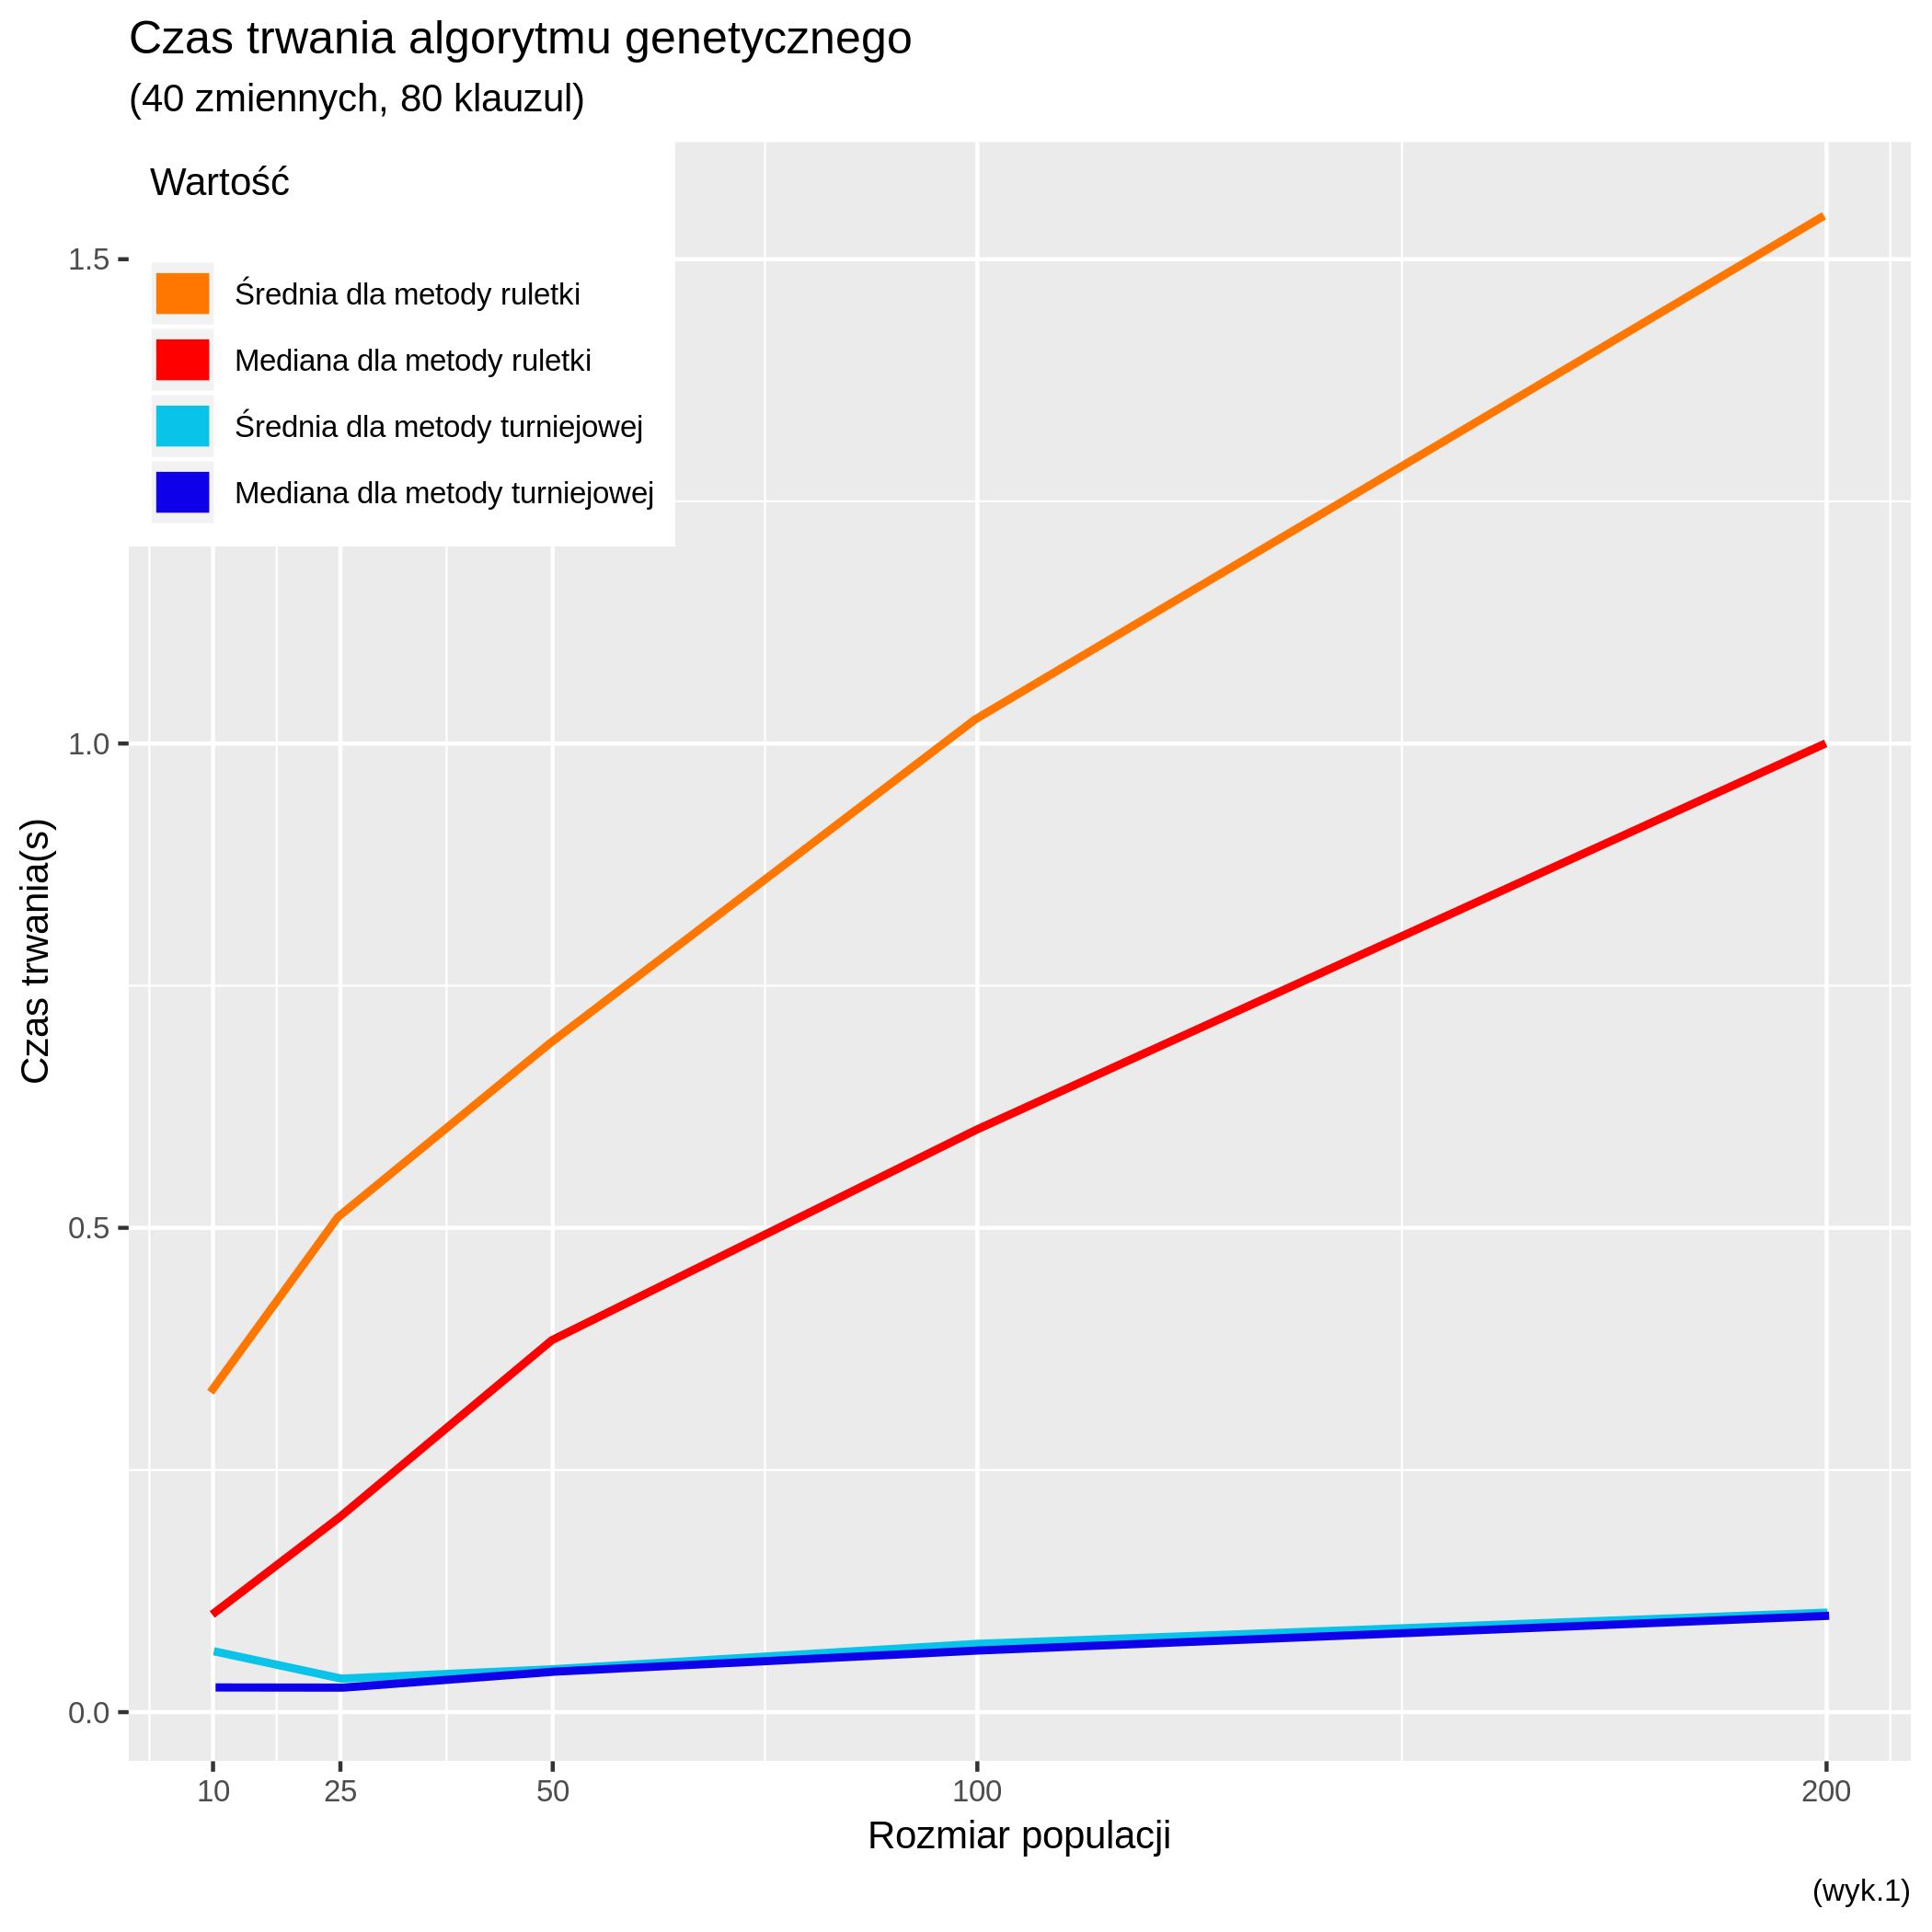
\includegraphics[width=\linewidth]{40x80k.png}
    \caption{Rysunek 1.1}
  \end{subfigure}
  \begin{subfigure}[b]{\linewidth}
    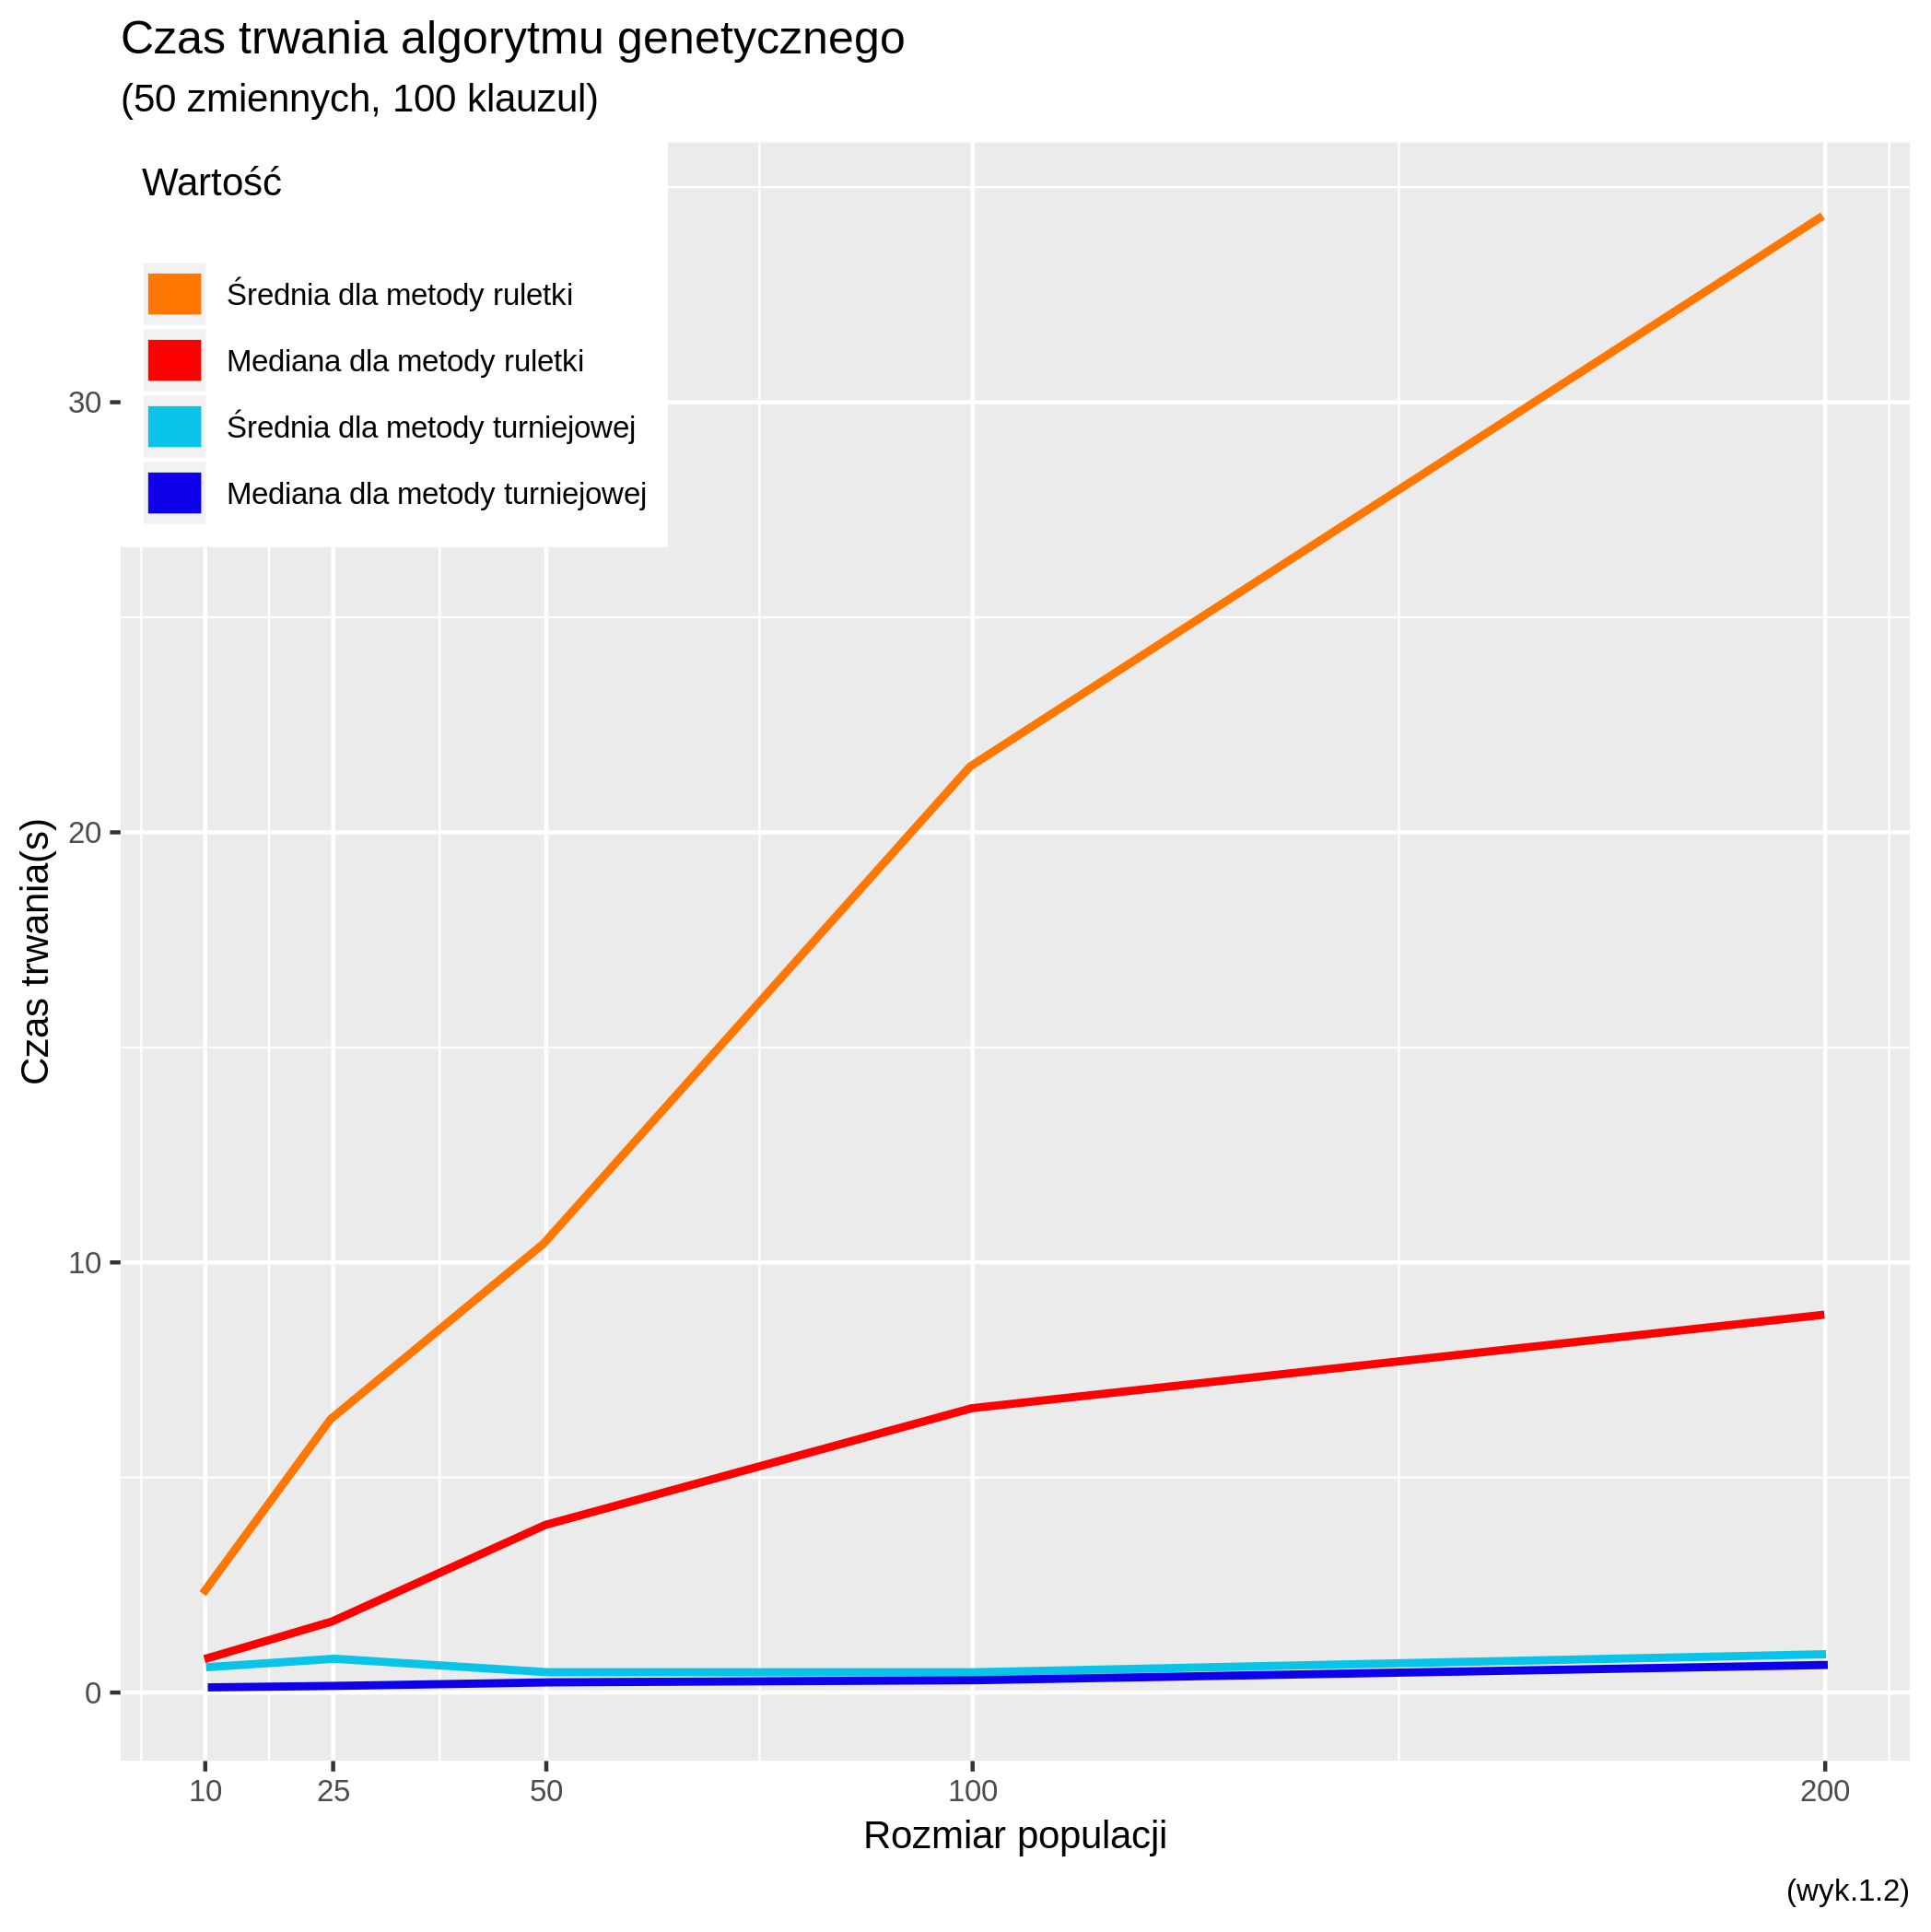
\includegraphics[width=\linewidth]{50x100k.png}
    \caption{Rysunek 1.2}
  \end{subfigure}
  \caption{Porównanie czasu trwania obliczeń dla dwóch instancji 3-SAT}
  \label{fig:coffee}
\end{figure}

\subsection{Rozmiar formuł}
Na wykresie \textit{(Rysunek 2)} został przedstawiony czas działania algorytmu dla zmieniających się rozmiarów klauzul. Zgodnie z oczekiwaniami czas potrzebny na wykonanie programu zwiększa się razem z rozmiarem rozwiązywanego problemu. Program nadzwyczajnie dobrze radzi sobie z problemami do rozmiarów 40 zmiennych w 80 klauzulach. Następnie zauważalny jest gwałtowny spadek wydajności rozwiązania oraz większa rozbieżność czasu wykonania pomiędzy uruchomieniami algorytmu. Możliwym rozwiązaniem tych zachwiań może okazać się dobór bardziej optymalnych parametrów. Natomiast czynnik losowości zmian bądź inny zestaw chromosomów początkowych może zaważyć o czasie zakończenia algorytmu, dlatego nie jest możliwe przewidzenie optymalnych parametrów dla danej instancji problemu bez wyczerpujących testów.
\begin{figure}[h!]
  \centering
    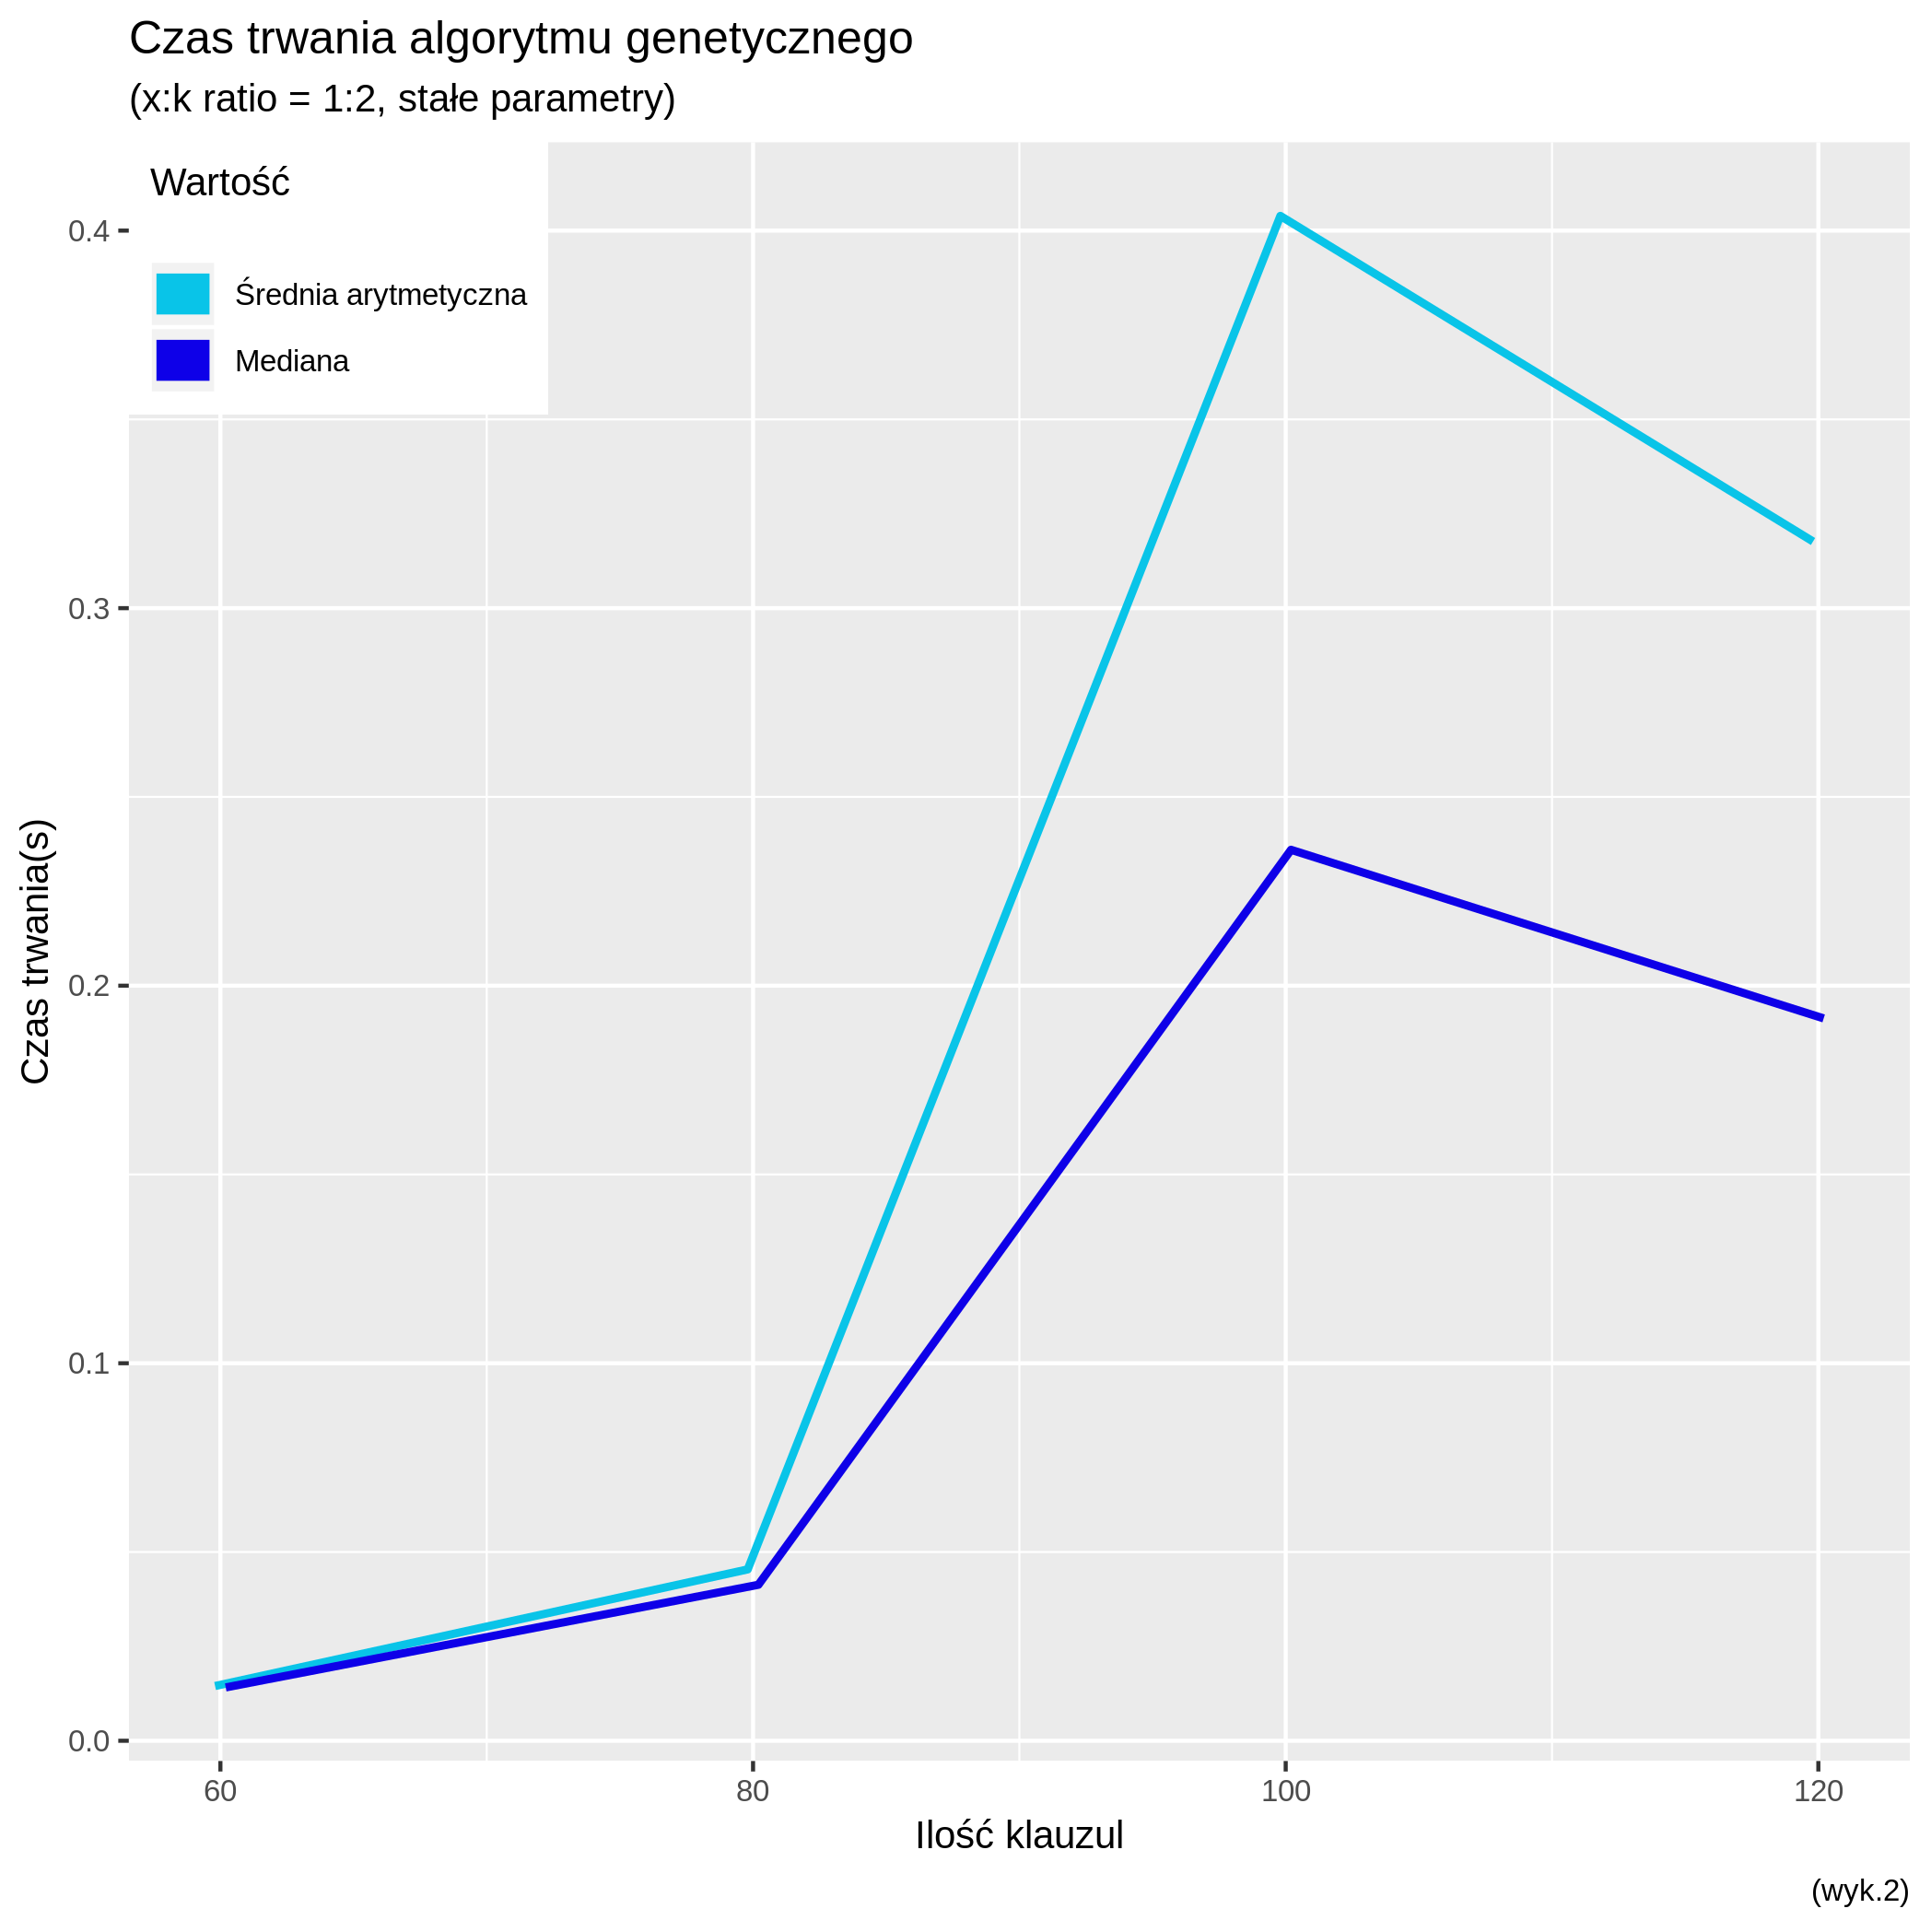
\includegraphics[width=\linewidth]{comp.png}
  \caption{Selekcja turniejowa dla różnych \\rozmiarów problemu}
  \label{fig:coffee}
\end{figure}

%----------------------------------------------------------------------------------------
%	REFERENCE LIST
%----------------------------------------------------------------------------------------

\begin{thebibliography}{99} % Bibliography - this is intentionally simple in this template

\bibitem[Zasoby online]{a}
\newblock {\em Algorytmy genetyczne }, dostęp online:
\newblock \url{http://home.agh.edu.pl/~vlsi/AI/gen_t/}
 
\bibitem[Zasoby online]{b}
\newblock {\em Introduction to Genetic Algorithm \& their application in data science }, dostęp online:
\newblock \url{https://www.analyticsvidhya.com/blog/2017/07/introduction-to-genetic-algorithm/} 

\bibitem[Kazuo Sugihara]{b}
\newblock {\em Measures for Performance Evaluation of Genetic Algorithms }, dostęp online:
\newblock \url{http://citeseerx.ist.psu.edu/viewdoc/download?doi=10.1.1.49.8611&rep=rep1&type=pdf} 
\end{thebibliography}

%----------------------------------------------------------------------------------------

\end{document}
